\documentclass[12pt]{article}

\usepackage{tikz}
\usepackage[ruled, vlined]{algorithm2e}
\usepackage{pst-node,pst-plot}
\usepackage{amsmath}
\usepackage{float}

\newcommand{\BigO}[1]{\ensuremath{\operatorname{\mathcal{O}}\bigl(#1\bigr)}}

\begin{document}
\title{Homework 12}
\author{Robbie McKinstry, Jack McQuown, Cyrus Ramavarapu}
\renewcommand{\today}{30 September 2016}
\renewcommand{\baselinestretch}{1.5}
\maketitle

\textbf{Please provide writing or oral feedback on this and future assignments.}

\section*{Dynamic Programming}
\subsection*{Problem 20: }
Given a series of $n$ points in the Euclidean plane labeled
$p_1,\dots,p_n$, dynammic programming can be used to find the 
minimum routing distance to service these points in order
with two tracers, $t_1$ and $t_2$.  In order tracing of these points
implies that if $p_j$ is serviced aftered $p_i$ by either tracer, it 
implies that $i<j$.\\\\
A dynamic programming algorithm for this problem can be
developed for this problem by initally considering all possible
routes the two tracers can take after each point is considered. 
This produces the following tree.
%Actually properly write out the tree.
\begin{center}
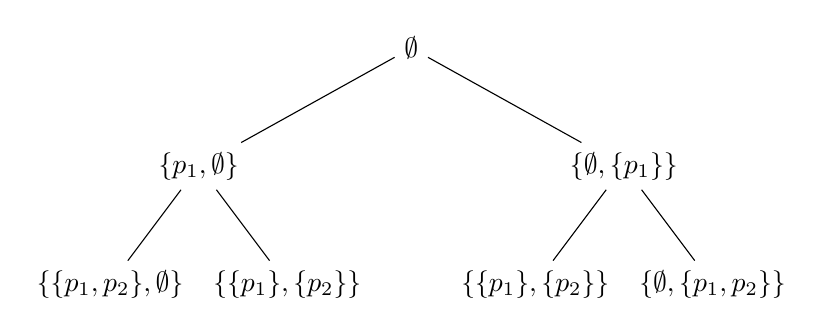
\begin{tikzpicture}[level distance=1.5cm,
    level 1/.style={sibling distance=5.40cm},
    level 2/.style={sibling distance=2.25cm},
    level 3/.style={sibling distance=1.85cm}]
    \node {$\emptyset$}
        child {node {${\{{p_1},\emptyset}\}$}
            child {node {${\{\{p_1,p_2\},\emptyset}$\}}}
            child {node {${\{\{p_1\},\{p_2\}\}}$}}
        }
        child {node {$\{{\emptyset,\{p_1\}\}}$}
            child {node {${\{\{p_1\},\{p_2\}\}}$}}
            child {node {$\{\emptyset,\{p_1,p_2\}\}$}}
        };
\end{tikzpicture}
\end{center} 
At every level in the tree a new point is considered and can be
taken by either $t_1$ or $t_2$.  However, if both $t_1$ and $t_2$
are considered in the tree, significant duplication is observed
at the leaves because the assignment of either $t_1$ or $t_2$ to
a set of points is arbitrary.  For example, if the information
in a leaf node is represented by the set ${pt_1,pt_2}$ where 
$pt_1$ and $pt_2$ are the sets of points visited respectively
by $t_1$ and $t_2$ then the node containing ${{p_1},{p_2,p_3}}$
is equivalent to the node containing ${{p_2,p_3},{p_1}}$.  This
is because the labels $t_1$ and $t_2$ do not really have meaning
and can be interchanged.  As a consequence of this result, half the
tree can be immediately eliminated.\\\\
Although removing half of the initial tree significantly reduces
the search space, the number of possible tours remaining is still
$2^{|P|-1}$, where $|P|$ is the number of points in the entire 
trace.  To further reduce the search space, two nodes at the same
level have both $t_1$ and $t_2$ respectively at the same point, then
the node with greater total distance traced can be pruned.  This is
a consequence that adding the next point to either node will result
in the same additional distance because the tracers $t_1$ and $t_2$
are respectively equividistant from the next point.  As a result
of this pruning rule, only the minimum of each combination of end points
such as $(p1,p2)$, needs to be kept at every level.  Applying this
rule to this problem produces the following algorithm, SlowPokeTaxi or
SPT\@.\\\\
\begin{algorithm}[H]
\SetKw{Func}{Function:}
\SetKw{Inp}{Input:}
\SetKw{Out}{Output:}
\SetKw{Glob}{Globals:}
\SetKw{Def}{Define:}
\SetKw{Ret}{Return:}
\Func{SlowPokeTaxi}\\
\Inp{$P={p_1,\ldots, p_2}$}\\
\Glob{$A[\ ][\ ][\ ]$}\\
\For{$i=0$ to $|P|$} {
    \For{$j=0$ to $|P|$} {
        \For{$k=0$ to $|P|$} {
            \If{$A[i][j][k]$ is defined} {
                $A[i+1][j][k] = \min(A[i+1][j][k], + A[i][j][k] + dist(j,i+1)$\\
                $A[i+1][j+1][k] = \min(A[i+1][j+1][k] + A[i][j+1][k] + dist(j,i+1)$\\
            }
        }
    }
}
\Ret{$\min(A[|P|][*][*])$}
\end{algorithm}
This algorithm runs in \BigO{n^3} because it has to consider all
possible available end points at a given level.  In this case
recovery of the actual sequence of traces requires determining
which point from the previous matches the difference in the 
distance between the current point and the previous.  This value
be subtracted from the currently minimum traversed values of $t_1$
and $t_2$.  Locating these values in the previous rows will 
determine which tracer covered this point.\\\\
This question now is if a faster algorithm can be developed.
By the will of Cthulhu, we found an algorithm can be
found to run in \BigO{n^2}.
It is believed that this algorithm can be developed by recognizing that
if two nodes contain information for $t_1$ and $t_2$ that are
end on respectively opposite points, the node with the longer
path can be pruned.  This results from the next point being
equal distance from both tracers in each case; however,
one tracer may have taken a longer route to the node.  Applying
this pruning rule gives the following algorithm.\\\\
\begin{algorithm}[H]
\SetKw{Func}{Function:}
\SetKw{Inp}{Input:}
\SetKw{Out}{Output:}
\SetKw{Glob}{Globals:}
\SetKw{Def}{Define:}
\SetKw{Ret}{Return:}
\Func{FastPokeTaxi}\\
\Inp{$P={p_1,\ldots, p_2}$}\\
\Glob{$A[\ ][\ ][\ ]$}\\
\For{$i=0$ to $|P|$} {
    \For{$j=0$ to $|P|$} {
        \tcc{$A[i][j][0]$ holds distance for $t_1$}
        \tcc{$A[i][j][1]$ holds distance for $t_2$}
        \If{$A[i][j][*]$ is defined} {
            \tcc{Add to $t_1$} 
            $A[i+1][j][0] = \min(A[i][j][0], A[i][j][0] + dist(j,i+1))$\\
            $A[i+1][j][1] = A[i+1][j][1]$\\
            \tcc{Add to $t_2$}
            $A[i+1][j+1][1] = \min(A[i][j+1][1], A[i][j][1] + dist(j,i+1))$\\
            $A[i+1][j][0] = A[i+1][j][0]$\\
        }
    }
}
\Ret{$\min(A[|P|][*][*])$}
\end{algorithm}
Since this algorithm only considers unique pairs and applies the pruning
rule regarding opposite endpoints on the same node, it runs in \BigO{n^2}.\\\\
To recover the exact sequence each tracer must travere, begin at the 
index where the minimum value was found. From this index find the difference
between points $n$ and the $n-1$.  This value can be subtracted from where the
minimum depending on whether the point was added to $t_1$ or $t_2$ to recover
the tracer of the previous point.  This processed can then be repeated for all
each previous $n$ up to the first point.
\subsection*{Problem 21: }

Since all points are colinear, any visit to a point $P_{i}$ if $P_{i} < 0 \implies \forall P_{j} : P_{i} < P_{j} < 0$, an optimal good path must visit $P_{j}$ before visiting $P_{i}$. This is obvious because any trip that skips over a point in between $P{i}$ and the origin would have to spend time traveling back to $P_{j}$, and this would increase the response time. An immediate corollary is that this is also true for all points farther along the real line in the positive direction as well.

Thus, an algorithm to find the optimal good path has one one choice: include in the path either the next point less than the current point, or the next point greater than the current point (colloquially, go left or go right). The search tree for an optimal good path can be represented as a tree of nodes storing a triple: the set of points unvisited on the left, the current position, and the set of points unvisited on the right. Each child node is populated by selecting either the greatest number of the left set (the first point on the left) or the least number in the second set (the first number on the right) and visiting that point. As a result, each parent has two children in the general case. When either set is empty, the remaining choices are obvious, and thus the node becomes a leaf. Without loss of generality, this occurs when the good path moves from the origin left $l$ times before moving right $r$ times, where $l$ is the total number of node left of the origin and $r$ is the total number of nodes right of the origin.

There are $l$ ways to move left before moving right (take the first point, take the first point and the second point, take the first point and ... and the $n$th point). Then, once moving right, there are $r$ ways to move right. Thus, there are $lr$ ways to move when changing direction no more than twice. The number of times you can change direction is limited the minimum of $l$ and $r$, since the number of times you can interleave right and left can not exceed the total number of times moving right and it cannot exceed the total number of times moving left. Assume $l$ is larger than $r$, without loss of generality. Then the total number of unique good paths is $l^{2}r$.

This leads to the following iterative algorithm:

Let $k$ be the minimum of $r$ and $l$. $\forall i < k$ consider changing direction $i$ times:

while $ k > 0$:
$\forall j < 1+ l - k$, go left $j$ times, before changing direction.
$\forall m < 1 + r - k$ go right $m$ times before changing direction.
Decrement $k$ by 1. Jump to the while condition.

\section*{Reduction}
\subsection*{Problem 1: }
In order to show that there is a {$O(n^2)$} time algorithm for matrix multiplication, it is first necessary to reduce matrix multiplication (MM) to lower triangle multiplication (LTM). Because we reduce matrix multiplication to LTM, we have an algorithm for MM and are stating that LTM is at least as hard as MM.\\\\
The reduction is as follows:\\

Transform matrices A and B into matrices C and D to use as input for LTM, which will take {$O(n^2)$} time.\\\\
$C = \begin{bmatrix}
0 & \frac{A}{3}\\[0.3em]
\frac{A}{3} & \frac{A}{3}
\end{bmatrix}$
$D = \begin{bmatrix}
0 & \frac{B}{3}\\[0.3em]
\frac{B}{3} & \frac{B}{3}
\end{bmatrix}$\\\\
Now from this transformed input, we can now use C and D in our LTM algorithm, which will also take {$O(n^2)$} time.\\\\
LTM(C,D) = $\begin{bmatrix}
\frac{AB}{9} & \frac{AB}{9}\\[0.3em]
\frac{AB}{9} & \frac{2AB}{9}
\end{bmatrix}$
=
{$\frac{1}{9}$} $\begin{bmatrix}
AB & AB\\[0.3em]
AB & 2AB
\end{bmatrix}$ \\\\
Get AB (the solution to MM(A,B)) from the above matrix in {$O(n^2)$} time\\\\
{return $AB$}\\\\
\noindent\rule{14cm}{0.4pt}\\\\
Therefore, because there is a {$O(n^2)$} time algorithm for lower triangle multiplication that is used in the matrix multiplication algorithm and every other step is also no more than {$O(n^2)$}, there is a {$O(n^2)$} time algorithm for matrix multiplication.
\end{document}
